\question{Коэффициент поглощения и усиления активной среды. Сечение
поглощения}

\subquestion{Коэффициент поглощения активной среды. Сечение поглощения.}
\begin{figure}[h]
    \center
    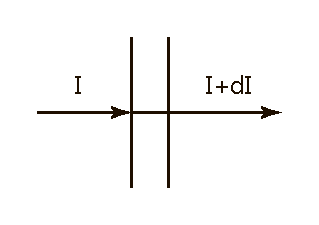
\includegraphics[width=.4\textwidth]{07_01}
\end{figure}
\[
    dI = -\alpha I dx
\]

Поглощение света в прозрачных средах носит резонансный характер. Энергия в
поглощенных фотонах пропорциональна количеству резонансных переходов
\[
    dI = W( n_2 - n_1 ) h\nu dx
\]
\[
    \frac{1}{\text{с}} \cdot \frac{1}{\text{м}^3} \cdot \text{Дж} \cdot \text{с}
        \cdot \frac{1}{\text{с}} \cdot \text{м} = \frac{\text{Вт}}{\text{м}^2}
\]
\[
    \alpha = \sigma( n_1 - n_2 )
\]

\emph{Сечение поглощения (эффективное сечение)} -- площадь поперечного сечения
такой области пространства вокруг частицы при пересечении с которой, фотон со
100\% вероятностью взаимодействует с ней.
\[
    \sigma = 10^{-14} \ldots 10^{-26} \text{ м}^2
\]
\[
    S_\text{ат.H} \sim 10^{-20} \text{ м}^2
\]

Зависимость коэффициента поглощения от насыщающего излучения
\begin{figure}[h]
    \center
    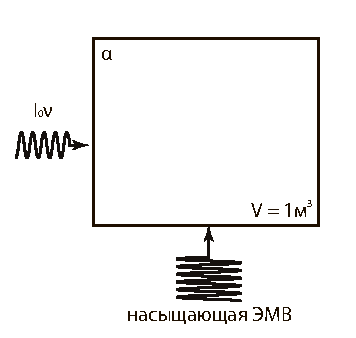
\includegraphics[width=.4\textwidth]{07_02}
\end{figure}
\[
\begin{array}{c}
    \D n = -\cfrac{n}{1+2W\tau} \\
    dI = W( n_2 - n_1 ) h\nu dx \\
    dI = -\alpha I dx \\
    \alpha = \sigma( n_1 - n_2 ) \\
    W = \cfrac{dI}{(n_2-n_1)h\nu dx} =
        \cfrac{-\alpha I dx}{(n_2-n_1)h\nu dx} =
        \cfrac{\sigma(n_2-n_1)I}{(n_2-n_1)h\nu} = \cfrac{\sigma I}{h\nu} \\
    W = \cfrac{\sigma I}{h\nu} \text{ -- вероятность индуцированных
        переходов}
\end{array}
\]

Введём величину:
\( I_s = \cfrac{h\nu}{2\sigma\tau}, \cfrac{\text{Вт}}{\text{м}^2} \)
\[
    I_s = I_s(\sigma,\tau,\nu)
\]
\[
    \frac{\D n}{n} = -\frac{1}{1+\cfrac{2\sigma I\tau}{h\nu}} =
        \frac{-1}{1+\cfrac{I}{I_s}}
\]
\( I_s \) -- интенсивность насыщения перехода, зависящая только от параметров
среды.

В случае резонансного поглощения \( \nu = \nu_0 \) получим зависимость:
\[
\begin{array}{c}
    \D n = \cfrac{-n}{1+\cfrac{I}{I_s}} \\
    n_1 - n_2 = \cfrac{n}{1+\cfrac{I}{I_s}} \quad\Big|\cdot\sigma \\
    \sigma(n_1-n_2) = \cfrac{n\sigma}{1+\cfrac{I}{I_c}} \rightarrow
        \alpha = \cfrac{\sigma n}{1+\cfrac{I}{I_s}}
\end{array}
\]

При \( I = 0 \rightarrow \alpha = \sigma n = \alpha_0 \). \( \alpha_0 \) --
коэффициент поглощения в отсутствие насыщающей ЭМВ или если она имеет другую
частоту \( \nu \neq \nu_0 \)

В реальности, частота насыщения волны не может быть равна частоте перехода,
всегда есть отклонение \( \pm\D\nu \), тогда коэффициент поглощения
определяется Лоренцевым форм-фактором.
\begin{figure}[h]
    \center
    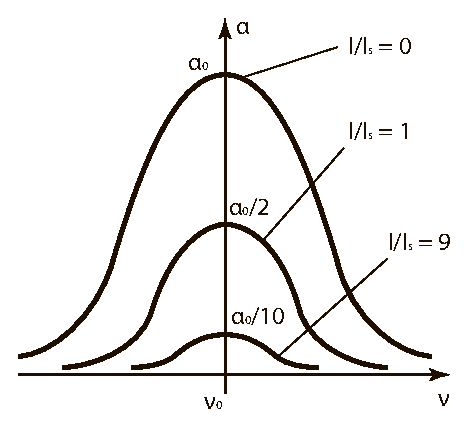
\includegraphics[width=.4\textwidth]{07_03}
\end{figure}

Вывод: при увеличении интенсивность насыщающего излучения коэффициент
поглощения уменьшается, а форма линий остаётся такой же, определяемая
однородным усилением.

\subquestion{Коэффициент усиления активной среды}
Поглощающая среда \( n_1 > n_2 \Rightarrow \alpha = \sigma(n_1 - n_2) > 0 \) \\
Усиливающая среда \( n_1 < n_2 \Rightarrow k = \sigma(n_2 - n_1) > 0 \) \\
где \( k \) -- коэффициент усиления.
\[
    k = \sigma(n_2 - n_1);\quad
    k = \frac{k_0}{1+\cfrac{I}{I_\sigma}}, \text{ где } k_0 \text{ при } I = 0
\]

\begin{figure}[h]
    \center
    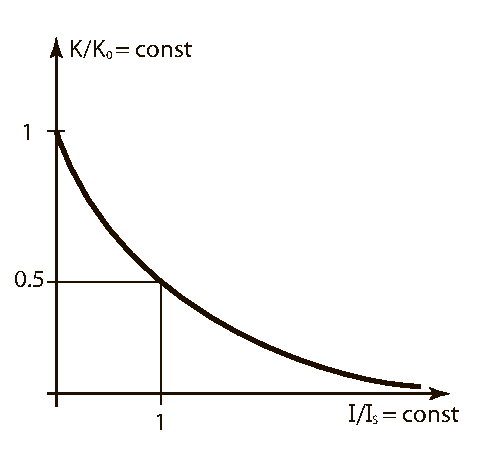
\includegraphics[width=.4\textwidth]{07_04}
\end{figure}

По мере роста интенсивности усиливающего излучения коэффициент излучения падет
и стремится к нулю.
